% Autor: Alfredo Sánchez Alberca (asalber@ceu.es)

\newproblem{tri-1}{gen}{}
%ENUNCIADO
{¿Es posible construir un triángulo de lados 70cm, 60cm y 100cm?
Justifica la respuesta.
}
%SOLUCIÓN
{Si.
}
%RESOLUCIÓN
{
}


\newproblem{tri-2}{gen}{}
%ENUNCIADO
{
Dado el siguiente triángulo rectángulo,

\begin{center}
\begin{tikzpicture}
\newcommand\XB{4}
\newcommand\ALPHA{30}
\newcommand\XC{\XB}
\newcommand\YC{{\XC*tan(\ALPHA)}}
% Draw the triangle
\draw  (0,0) coordinate (A) -- (\XC,\YC) coordinate (C) -- (\XB,0) coordinate (B) -- (0,0);
% Draw nodes
\node at (A)[anchor=north] {A};
\node at (B)[anchor=north] {B};
\node at (C)[anchor=south] {C};
% Draw edge text
\node (c) at ($(A)!0.50!(B)$) [below] {8};
\node (b) at ($(A)!0.50!(C)$) [above,rotate=\ALPHA] {10};
%\node (a) at ($(B)!0.5!(C)$) [right] {5};
% draw angles
\draw (0,0) -- (0:0.75cm) arc (0:\ALPHA:.75cm);
\coordinate[label=right:$\alpha$] (Alpha) at (0.25,0.15);
\begin{scope}[shift={(\XB,0)}]
\draw (-0.5,0) |- (0,0.5);
\draw (150:0.35cm) node {$\beta$};
\end{scope}
\begin{scope}[shift={(\XC,\YC)}]
\draw (0,0) -- ({180+\ALPHA}:0.5cm) arc ({180+\ALPHA}:{270}:0.5cm);
\draw (-0.2,-0.05) node[below] {$\gamma$};
\end{scope}
\end{tikzpicture}
\end{center}

\begin{enumerate}
\item Calcular sus ángulos en radianes.
\item Calcular el valor del lado $BC$.
\end{enumerate}
}
%SOLUCIÓN
{\begin{enumerate}
\item $\alpha=0.64$ rad, $\beta=\pi/2$ rad y $\gamma=0.93$ rad.
\item $6$.
\end{enumerate}
}
%RESOLUCIÓN
{
}


\newproblem{tri-3}{gen}{}
%ENUNCIADO
{
Dado el siguiente triángulo rectángulo,
\begin{center}
\begin{tikzpicture}
\newcommand\XB{4}
\newcommand\ALPHA{30}
\newcommand\XC{\XB}
\newcommand\YC{{\XC*tan(\ALPHA)}}
% Draw the triangle
\draw  (0,0) coordinate (A) -- (\XC,\YC) coordinate (C) -- (\XB,0) coordinate (B) -- (0,0);
% Draw nodes
\node at (A)[anchor=north] {A};
\node at (B)[anchor=north] {B};
\node at (C)[anchor=south] {C};
% Draw edge text
\node (b) at ($(A)!0.50!(C)$) [above,rotate=\ALPHA] {8};
% draw angles
\draw (0,0) -- (0:1cm) arc (0:\ALPHA:1cm);
\coordinate[label=right:$30º$] (Alpha) at (0.25,0.15);
\begin{scope}[shift={(\XB,0)}]
\draw (-0.5,0) |- (0,0.5);
\draw (150:0.35cm) node {$\beta$};
\end{scope}
\begin{scope}[shift={(\XC,\YC)}]
\draw (0,0) -- ({180+\ALPHA}:0.5cm) arc ({180+\ALPHA}:{270}:0.5cm);
\draw (-0.2,-0.05) node[below] {$\gamma$};
\end{scope}
\end{tikzpicture}
\end{center}

\begin{enumerate}
\item Calcular el ángulo $\gamma$ en radianes.
\item Calcular la longitud de sus lados $AB$ y $BC$.
\item Calcular su área.
\end{enumerate}

}
%SOLUCIÓN
{\begin{enumerate}
\item $\gamma=60$ rad.
\item $|AB|=6$ y $|BC|=\sqrt{48}$.
\item $3\sqrt{48}$.
\end{enumerate}
}
%RESOLUCIÓN
{
}


\newproblem{tri-4}{gen}{}
%ENUNCIADO
{
Calcular la longitud de los lados del triángulo rectánculo siguiente si el área es 25.
\begin{center}
\begin{tikzpicture}
\newcommand\XB{2}
\newcommand\ALPHA{60}
\newcommand\XC{\XB}
\newcommand\YC{{\XC*tan(\ALPHA)}}
% Draw the triangle
\draw  (0,0) coordinate (A) -- (\XC,\YC) coordinate (C) -- (\XB,0) coordinate (B) -- (0,0);
% Draw edge text
\node (c) at ($(A)!0.50!(B)$) [below] {$x$};
\node (b) at ($(A)!0.50!(C)$) [above,rotate=\ALPHA] {$h$};
\node (a) at ($(B)!0.5!(C)$) [right] {$2x$};
% draw angles
\begin{scope}[shift={(\XB,0)}]
\draw (-0.5,0) |- (0,0.5);
\end{scope}
\end{tikzpicture}
\end{center}

}
%SOLUCIÓN
{$x=5$ y $h=5\sqrt{5}$.
}
%RESOLUCIÓN
{
}


\newproblem*{tri-5}{gen}{}
%ENUNCIADO
{
Dado el siguiente triángulo,
\begin{center}
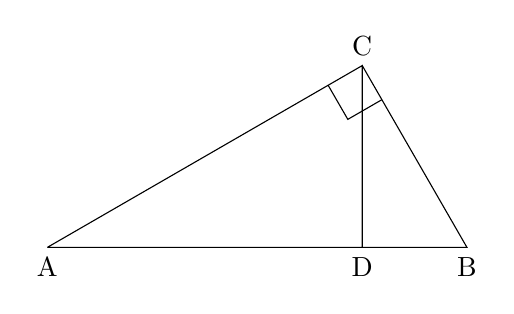
\begin{tikzpicture}
\newcommand\XB{4}
\newcommand\ALPHA{30}
\newcommand\XC{\XB}
\newcommand\YC{{\XC*tan(\ALPHA)}}
% Draw the triangle
\draw  (0,0) coordinate (A) -- (\XC,\YC) coordinate (C) -- (\XB,0) coordinate (B) -- (0,0);
\draw (B) -- (\XB+1.33,0) coordinate (D) -- (C);
% Draw nodes
\node at (A)[anchor=north] {A};
\node at (B)[anchor=north] {D};
\node at (C)[anchor=south] {C};
\node at (D)[anchor=north] {B};
% draw angles
\begin{scope}[shift={(\XC,\YC)}]
\draw[rotate=120] (-0.5,0) |- (0,0.5);
\end{scope}
\end{tikzpicture}
\end{center}

demostrar las siguientes igualdades:
\begin{enumerate}
\item $\dfrac{AD}{CD}=\dfrac{CD}{DB}$.
\item $AC^2= AB\cdot AD$.
\item $BC^2= AB\cdot DB$.
\item $AC^2 + BC^2= AB^2$ (teorema de Pitágoras).
\end{enumerate}

}
%SOLUCIÓN
{
}
%RESOLUCIÓN
{
}


\newproblem{tri-6}{gen}{}
%ENUNCIADO
{
Desde un barco se avista la luz de un faro sobre un acantilado con un ángulo de 30º sobre la línea del horizonte, y tras alejarse 1 km el ángulo de la visual es de 10º.
¿A qué altura sobre el nivel del mar está la luz del faro?
}
%SOLUCIÓN
{$250$ m.
}
%RESOLUCIÓN
{
}


\newproblem{tri-7}{gen}{}
%ENUNCIADO
{
Desde lo alto de un edificio de 100 metros se observa la base de otro edificio con un ángulo de 20º y su punto más alto con un ángulo de 10 grados.
¿Cuál es la altura de segundo edificio?
}
%SOLUCIÓN
{$148.45$ m.
}
%RESOLUCIÓN
{
}


\newproblem{tri-8}{gen}{}
%ENUNCIADO
{
En el siglo III a.C. Eratóstenes observó que en su ciudad Syene los rayos del sol no provocaban sombra alguna sobre un obelisco. 
Más tarde, el mismo día y a la misma hora observó que en Alejandría los rayos del sol proyectaban una sombra de $1.263$ m al caer sobre un obelisco de 10 m. 
Calcular el radio de la tierra con estos datos, sabiendo que la distancia entre Syene y Alejandría en línea recta es de 800 km aproximadamente. 
}
%SOLUCIÓN
{$6366$ m.
}
%RESOLUCIÓN
{
}


\newproblem{tri-9}{gen}{}
%ENUNCIADO
{Un avión se aproxima al aeropuerto de aterrizaje con un una altura de  avión se encuentra a una altura de 1500 metros. 
Desde lo alto de la torre de control se observa el avión con un ángulo de 30º sobre la horizontal. 
¿A qué distancia se encuentra el avión de la base de la torre de control si la torre mide 50 m?
}
%SOLUCIÓN
{$6366$ m.
}
%RESOLUCIÓN
{$2925.32$ m.
}


\newproblem{tri-10}{gen}{}
%ENUNCIADO
{
Dado el siguiente triángulo,
\begin{center}
\begin{tikzpicture}
  \newcommand\XB{5}
  \newcommand\ALPHA{30}
  \newcommand\XC{{(\XB*(cos(\ALPHA)*cos(\ALPHA) - sin(\ALPHA)*sin(\ALPHA)) + \XB)*0.5}}
  \newcommand\YC{{sqrt(cos(\ALPHA)*\XB*cos(\ALPHA)*\XB - (\XB*(cos(\ALPHA)*cos(\ALPHA) - sin(\ALPHA)*sin(\ALPHA)) + \XB)*0.5*(\XB*(cos(\ALPHA)*cos(\ALPHA) - sin(\ALPHA)*sin(\ALPHA)) + \XB)*0.5)}}
  % Draw the triangle
  \draw (0,0) coordinate (A) -- (\XC,\YC) coordinate (C) -- (\XB,0) coordinate (B) -- (0,0);
  % Draw edge text
  \node (c) at ($(A)!0.5!(B)$) [below] {10};
  \node (b) at ($(A)!0.5!(C)$) [above] {b};
  \node (a) at ($(B)!0.6!(C)$) [right] {6};
  % draw angles
  \draw (0,0) -- (0:0.75cm) arc (0:\ALPHA:.75cm);
  \coordinate[label=right:$\alpha$] (Alpha) at (0.25,0.15);
  \begin{scope}[shift={(\XB,0)}]
      \draw(0,0) -- (-180:0.50cm) arc (180:{180-(90-\ALPHA)}:0.5cm);
      \draw (150:0.35cm) node {$\beta$};
  \end{scope}
  \begin{scope}[shift={(\XC, \YC)}]
      \draw (0,0) -- ({180+\ALPHA}:0.5cm) arc ({180+\ALPHA}:{180+\ALPHA+90}:0.5cm);
      \draw (-0.1,-0.05) node[below] {$80º$};
  \end{scope}
\end{tikzpicture}
\end{center}

\begin{enumerate}
  \item Calcular los ángulos $\alpha$, $\beta$ y el lado $b$.
  \item Calcular su área. 
\end{enumerate}
}
%SOLUCIÓN
{\begin{enumerate}
  \item $\alpha=36.22º$, $\beta=63.78º$ y $b=9.11$.
  \item $26.91$.
\end{enumerate}
}
%RESOLUCIÓN
{
}


\newproblem{tri-11}{gen}{}
%ENUNCIADO
{
Dado el siguiente triángulo,
\begin{center}
\begin{tikzpicture}
  \newcommand\XB{5}
  \newcommand\ALPHA{30}
  \newcommand\XC{{(\XB*(cos(\ALPHA)*cos(\ALPHA) - sin(\ALPHA)*sin(\ALPHA)) + \XB)*0.5}}
  \newcommand\YC{{sqrt(cos(\ALPHA)*\XB*cos(\ALPHA)*\XB - (\XB*(cos(\ALPHA)*cos(\ALPHA) - sin(\ALPHA)*sin(\ALPHA)) + \XB)*0.5*(\XB*(cos(\ALPHA)*cos(\ALPHA) - sin(\ALPHA)*sin(\ALPHA)) + \XB)*0.5)}}
  % Draw the triangle
  \draw (0,0) coordinate (A) -- (\XC,\YC) coordinate (C) -- (\XB,0) coordinate (B) -- (0,0);
  % Draw edge text
  \node (c) at ($(A)!0.5!(B)$) [below] {c};
  \node (b) at ($(A)!0.5!(C)$) [above] {8};
  \node (a) at ($(B)!0.6!(C)$) [right] {5};
  % draw angles
  \draw (0,0) -- (0:0.75cm) arc (0:\ALPHA:.75cm);
  \coordinate[label=right:$\alpha$] (Alpha) at (0.25,0.15);
  \begin{scope}[shift={(\XB,0)}]
      \draw(0,0) -- (-180:0.50cm) arc (180:{180-(90-\ALPHA)}:0.5cm);
      \draw (150:0.35cm) node {$\beta$};
  \end{scope}
  \begin{scope}[shift={(\XC, \YC)}]
      \draw (0,0) -- ({180+\ALPHA}:0.5cm) arc ({180+\ALPHA}:{180+\ALPHA+90}:0.5cm);
      \draw (-0.1,-0.05) node[below] {$80º$};
  \end{scope}
\end{tikzpicture}
\end{center}

\begin{enumerate}
  \item Calcular los ángulos $\alpha$, $\beta$ y el lado $c$.
  \item Calcular su área. 
\end{enumerate}
}
%SOLUCIÓN
{\begin{enumerate}
  \item $\alpha=42.96º$, $\beta=57.04º$ y $b=8.67$.
  \item $18.18$.
\end{enumerate}
}
%RESOLUCIÓN
{
}